\chapter{Optimizers} % (fold)
\label{cha:optimizers}
	\section{Stochastic Gradient Descent} % (fold)
	\label{sec:sgd}
		When choosing an optimizer, the \textit{Stochastic Gradient Descent}, SGD for short, is a quite common
		choice. It is not the best though, since, as proved by the last developments in the machine learning
		field, its convergence's rate is quite slow. 
		Said that, it is also true that it allows to finds a very low value of the cost function quickly enough. 

		The algorithm \ref{alg_sgd} is the standard SGD version implemented, as described in
		\cite{Goodfellow-et-al-2016}, supporting both \textit{momentum} and \textit{regularization}.
		\cite{LIVIERIS2013491}

		SGD is an extension of the \textit{gradient descent algorithm}(GD). It is an iterative first-order optimization technique, usefull to minimize the objective loss function: the main goal is, indeed, to identify and compute a local minimum, moving along the direction of the steepest descent of the function, that is the negative gradient $-\nabla\mathcal{E}(\textbf{W})$.

		As we already said, the objective of the training procedure is to minimize the loss function. Of course, in order to arrive to a local minimum, it is necessary to update the synaptic weights \textbf{W} at every iteration as $\textbf{W} = \textbf{W} +\Delta \textbf{W}$.

		The correction applied to the weights is defined as follows, taking a step in the opposite direction of the cost gradient:
		\begin{equation}
			\label{delta_rule}
			\Delta w_{ji}(n) = -\eta \frac{\partial\mathcal{E}(n)}{\partial w_{ji}(n)},
		\end{equation}

		where $\eta$ is the learning rate. The latter one is a fundamental hyperparameters which has to been choosen wisely, since it represents how much is right to move along the descent direction: too much and the procedure will be vain, missing the minimum; too little and the converge will be slow.

		Unlike the GD algorithm, that could be quite costly because of the potentially big number of training examples, getting a longer time to converges to the minimum when dealing with a very large dataset, the SGD algorithm requires only the evaluation of one example for epochs (on-line mode).

		Here, however, we refer to SGD even when using the entire or just a subset of training examples to be considered at each epoch of training (batch or mini batch).

		The name stochastic derives from the fact that the samples are selected randomly, bringing to an approximation of the true gradient estimated using a small set of samples. This is also the reason of the typical zig-zag pattern in the path towards the minimum of the loss function, as visible in fig.\ref{fig:gradient}.
		\begin{figure}
			\centering
		    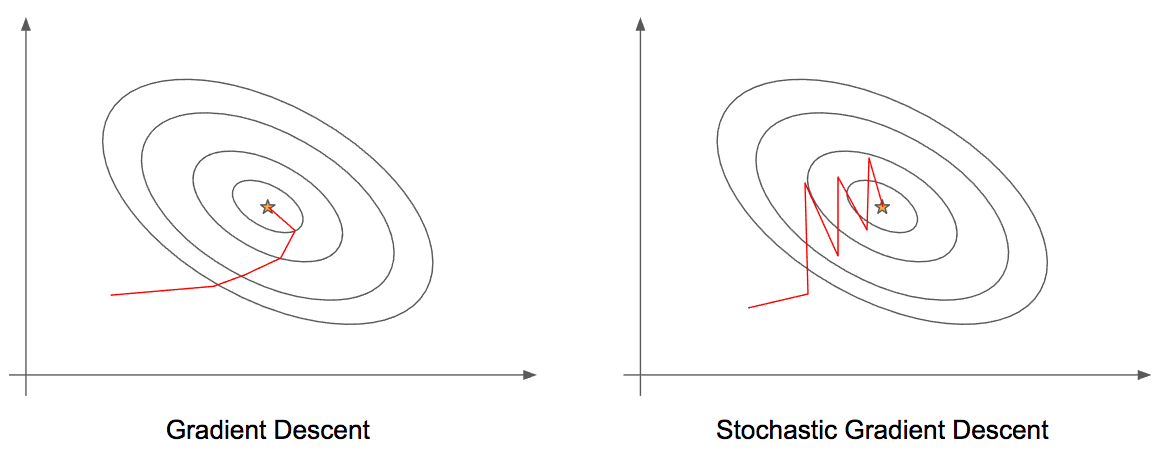
\includegraphics[width=.8\linewidth, scale=0.7]{img/figures/gradient.png}
			\caption{The different trajectories from GD and SGD.}
			\label{fig:gradient}
		\end{figure}
		%Due to its stochastic nature, c. However, it has been shown that SGD almost surely converges to the global cost minimum if the cost function is convex (or pseudo-convex)[1] [1] Bottou, Léon (1998). "Online Algorithms and Stochastic Approximations". Online Learning and Neural Networks. Cambridge University Press. ISBN 978-0-521-65263-6
		
		For what concernes the the convergence of the stochastic gradient descent algorithm, it depends on the choice of $\eta$: it is necessary to gradually decrease the learning rate over the epochs for ensure convergence.
%deeplearning
		A sufficient condition to guarantee convergence of SGD is that the sequence of decreasing learning rates satisfy:

		\begin{equation}
			\label{delta}
			\sum_{t=1}^\infty \eta_t = \infty \text{  } \text{ and }\text{  } \sum_{t=1}^\infty \eta_t^2 < \infty 
		\end{equation}

		Futhermore, if we assume that the Hessian matrix of the loss function is strictly positive definite at the optimum, that is having the loss function is strogly convex, the convergence rate is $O(\frac{1}{k})$, with \textit{k} as the number of epochs in the training. %strongly convex
		Otherwise, relaxing this assumption in presence of a convex problem, the convergence rate becomes $O(\frac{1}{\sqrt[]{k}})$\cite{Goodfellow-et-al-2016}.%Bottou L. (2012) Stochastic Gradient Descent Tricks. In: Montavon G., Orr G.B., Müller KR. (eds) Neural Networks: Tricks of the Trade. Lecture Notes in Computer Science, vol 7700. Springer, Berlin, Heidelberg

		A property of SGD is that computation time per update does not grow with the number of training examples, allowing convergence even in presence of a large dataset.

		\subsection{Momentum} % (fold)
		\label{sec:momentum}
			When computing the adjustment of the synaptic weights $\Delta\textbf{W}$ as in Eq. \ref{delta}, the choice of the learning rate $\eta$ influences the convergence of the SGD algorithm.
			The smaller is $\eta$, the smaller will be the changes in the matrix of weights and the rate of learning, but the smoother will be the trajectory.

			On the contrary, a bigger $\eta$ will bring to a faster convergence, but also to an oscillatory behaviour.

			A way to accelerate the SGD is the use of the \textit{Classical Momentum} (CM), a first order optimization technique which accelerate gradient descent, and so the learning rate of the final training.

			It consists in the adjustment of the new weigths through a velocity vector \textbf{v} that accumulates the gradient elements in the directions of reduction of the loss function \ref{loss} and a momentum coefficient $\alpha \in [0,1]$: the larger is  $\alpha$, the more the previous gradients affect the current direction.

			In this case, the classical momentum is given by:

			\begin{equation}
				\label{classical_momentum}
				\textbf{v}_k = \alpha\textbf{v}_{k-1} + \eta\nabla\mathcal{E}(\textbf{W}_k).
			\end{equation}

			The new synaptic weights are then updated as:
			\begin{equation}
				\label{update_momentum}
				\textbf{W}_k = \textbf{W}_{k-1}  + \textbf{v}_k.
			\end{equation}

			A variant of the CM algorithm, is the \textit{Nesterov's Accelerated Gradient} (NAG), which allows to avoid the oscillatory behaviour in the trajectory computed with CM, as visible in fig.\ref{fig:momentum_graph}%fig2 on the importance}. 

			The velocity vector \textbf{v} is computed as:

			\begin{equation}
				\label{nesterov_momentum}
				\textbf{v}_k = \alpha\textbf{v}_{k-1} + \eta\nabla\mathcal{E}(\textbf{W}_k + \alpha\textbf{v}_{k-1}).
			\end{equation}
			
			The update of the weights \textbf{W} follows the one described in Eq. \ref{update_momentum}.

			The variant respect Eq. \ref{classical_momentum}, shown in fig.\ref{fig:momentum}, is given by the fact that the gradient $\nabla\mathcal{E}$ is evaluated after the current velocity is applied: NAG first update the $\textbf{W}_k$, making a jump in the direction of the previous accumulated gradient, and then evaluate the gradient in that point and makes a correction. This procedure allows it to change velocity vector $\textbf{v}_{k}$ in a faster way.

			It's worth to underline that, in case of batch mode and convex functions, Nesterov momentum brings the rate of convergence from $O(\frac{1}{k})$ (after k steps) to $O(\frac{1}{k^2})$. % Nesterov (1983).
			\begin{figure}
			\centering
			  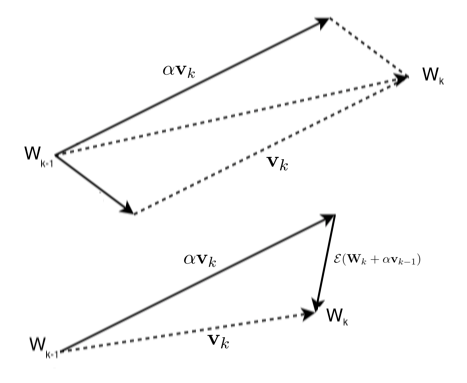
\includegraphics[width=.4\linewidth, scale=0.5]{img/figures/momentum}
			  \caption{The classical momentum on top and the Nesterov Accelerated gradient on bottom.}
			  \label{fig:momentum}

			  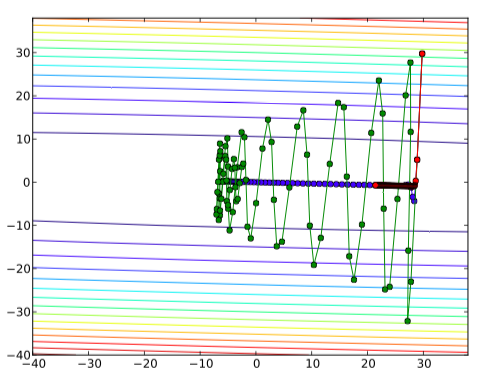
\includegraphics[width=.4\linewidth, scale=0.5]{img/figures/momentum_graph}
			  \caption{The trajectory from CM (in green) and the one from NAG (in blue).}
			  \label{fig:momentum_graph}
			\end{figure}


		\subsection{Regularization} % (fold)
		\label{sec:regularization}

			In order to garantee a tradeoff between goodness and complexity of the model, the regularization is allowed in the network. This choice is important to ensure that the model doesn't grow too much in complexity. 

			Regularization, in fact, adds a penalty as the model's complexity increases, forcing some weights to take values close to zero,  if they have little influence on the newtork performance and so resulting in poor generalization.

			It basically modifies the objective loss functions as follows:
			
			\begin{mini}
			  {\textbf{W}\in \mathbb{R}^n}{\mathcal{E}(\textbf{W}) + \lambda\mathcal{E}_c(\textbf{W}),}{}{}
			\end{mini}

			where $\mathcal{E}_c(\textbf{W})$ is a complexity penalty term based of the weights, and $\lambda$ is a parameter which tells how much importance must have the complexity penalty term.

			Two kinds of regularization are implemented:

			\begin{itemize}
				\item \textit{L1}: also called Lasso Regression, which results in $\mathcal{E}_c(\textbf{W}) = \sum_{i=1}^{k} |w_i| = \|\textbf{W}\|_1$;
				\item \textit{L2}: also known as Ridge Regression, which results in $\mathcal{E}_c(\textbf{W}) = \sum_{i=1}^{k}w_i^2 = \|\textbf{W}\|_2^2$.
			\end{itemize}




	\section{Nonlinear Conjugate Gradient} % (fold)
	\label{sec:nonlinear_conjugate_gradient}

		An intresting optimization ables to lead to an improvement of the performances of the Neural Network, is the use of high-order information during the training phase.

		We can, indeed, approximate the \textit{loss function} in a quadratic form, around a given point \textbf{W}, using the Taylor approximation:

		 \begin{equation}
		 	\label{quadratic}
		    \mathcal{E}(\textbf{W} + \Delta\textbf{W}) = \mathcal{E}(\textbf{W})+\textbf{g}\mathcal{E}^T\Delta\textbf{W}+ \frac{1}{2}\Delta\textbf{W}^T\textbf{H}\Delta\textbf{W},
		 \end{equation}

		where \textbf{H} is the \textit{Hessian} matrix and \textbf{g} the gradient vector, getting the benefit of choosing the search direction and the step size more carefully by using information from the second order approximation.

		Given Eq. \ref{quadratic}, the optimum adjustment to apply to the weights of the network should be
 		\begin{equation}
		 	\label{weight_star}
			\Delta\textbf{W}^* = \textbf{H}^{-1}\textbf{g},
		\end{equation}

		carrying the weight of the computation of the inverse of the Hessian.

		In order to avoid this expensive computation, we can use the \textit{Conjugate Gradient} methods, which are a class of iterative second-order optimization methods, derived from the steepest-descent algorithm, that ensure low memory requirements.

		In this way, the adjustment to the synaptic weights of the network is computed as:
		 \begin{equation}
		 	\label{weight}
		    \Delta\textbf{W} = \alpha\textbf{d},
		 \end{equation}
		where $\alpha$ is the learning rate and \textbf{d} is the new direction found.

		In our case, the nonlinear conjugate gradient methods are designed to solve the following minimization problem:

		\begin{mini}
		  {\textbf{W}\in \mathbb{R}^n}{\mathcal{E}(\textbf{W}),}{}{}
		\end{mini}

		where $\mathcal{E}$ is the loss function and \textbf{W} are the synaptic weights of the network.

		As showed in the pseudocode \ref{cgd}, the iterative formula generates a sequence of weights $\{W_k\}$, for every epoch of training \textit{k}, as:

		\begin{equation}
			\textbf{W}_{k+1} = \textbf{W}_{k} + \alpha\textbf{d}_k, \text{  }\text{  }\text{  } \textit{k} = 0,1,...,
		\end{equation}

		where $\alpha_k$ is a learning rate and $\textbf{d}_k$ is a descent direction. These are the new synaptic weights computed with the adjustment of eq.\ref{weight}.

		% Because the error function E(~,) is nonquadratic, the algorithm will not necessarily con- verge in N steps. If the algorithm has not converged after N steps, the algorithm is restarted, i.e., initializing fik+J to the current steepest descent direction ~k+~  A Scaled Conjugate Gradient Algorithm for Fast Supervised Learning p4


		\subsection{Search Direction}
		\label{sub:search_direction}
			The direction $\textbf{d}_k$ holds the sequent property:
			\begin{equation}
			\textbf{d}_k^T\textbf{H}\textbf{d}_{tk-1} = 0,
			\end{equation}

		 	that means it is conjugate to the previous direction $\textbf{d}_{k-1}$. Furthermore, it doesn't need to know all the 	previous directions, but it only needs the last one, which is why it requires very little storage and computation.

			When dealing with quadratic functions, this method keeps the progress obtained so far in the minimization of the loss function, by ensuring that the gradient along the previous direction does not increase.
			Anyway, it's worth to underline that this method can also be applyed with nonlinear functions: in this case, it should be necessary to restart the process, since there is no assumption that the conjugate directions previously found are still at the minimum of the function.

			Each new direction it's a linear combination of the steepest descent -\textbf{g} and the previous direction $\textbf{d}_{k-1}$, and it is defined as:
			\begin{equation}
			\label{dir}
			  \textbf{d}_k=\begin{cases}
			    -\textbf{g}_0, & \text{if $k=0$};\\
			    -\textbf{g}_k + \beta_k\textbf{d}_{k-1}, & \text{otherwise,}
			  \end{cases}
			\end{equation}

			where $\beta_k$ is a scalar, to be determined, that says how much of the previous direction should be added to the newest one. When applied to minimize a strictly convex quadratic function, it ensure that the directions $\textbf{d}_{k}$ and $\textbf{d}_{k-1}$ are conjugate with respective to the Hessian of the objective function, that is the property \ref{sub:search_direction} holds.

			Of course, the first search direction when $k = 0$ is defined as the steepest descent direction at the initial weight $\textbf{W}_0$ while, for $k > 1$, a minimization along each of the search direction is performed.

			Since it may be that the direction found is not a descent direction of the objective function, another modified search direction, proposed by Zang et al.\ref{zhang}, has been tested in the project. It ensures sufficient descent $g_k^T = -\|g_k\|^2$, indipendent of the line search used or the convexity of the objective function, and is defined as follows:

			\begin{equation}
			\label{mod_dir}
				\textbf{d}_k^+=\begin{cases}
			    -\textbf{g}_0, & \text{if $k=0$};\\
			    -(1 + \beta_k\frac{\textbf{g}_k^T\textbf{d}_{k}}{\|\textbf{g}_k\|})\textbf{g}_k + \beta_k\textbf{d}_{k-1}^+, & \text{otherwise.}
			  \end{cases}
			\end{equation}



		\subsection{Beta}
		\label{sub:beta}
			What really makes the difference in the computation of the conjugate gradient algorithm, is the choice of the method used to compute the $\beta$ coefficient.

			In fact, there has been proposed various choices for computing it, each one giving different efficiency and properties.

			The formulas tested in our implementation are four: the Fletcher-Reeves (FR), the Polak-Ribierère (PR), the Hestenes-Stiefel (HS) and a Modified Hestenes-Stiefel ($MHS^+$).

			One of the properties that must be garanteed, is the global convergence of the method. Since, in our network, we are dealing with a nonquadratic loss function, the direction computed as in eq. \ref{dir} could not be a descent direction. In order to avoid this issue, all the methods have been modified as follows, ensuring the global convergence:
			\begin{equation}
			\label{beta_max}
				 \beta^+ = max\{\beta, 0\}.
			\end{equation}

			This change provides a sort of restart of the algorithm, in case the $\beta$ found is negative. This is equivalent to forget the last search direction and start again the search from the steepest descent direction. Furthermore, because of the nonquadratic nature of the error function, the algorithm will not necessarily converge in N steps, as it usually does when applied to quadratic functions. The use of $\beta$ in eq. \ref{beta_max} is similar to adopt the strategy of restarting the algorithm after N steps, initializing $d_k$ to the current steepest descent direction.% A Scaled Conjugate Gradient Algorithm for Fast Supervised Learning p4

			\begin{equation}
			\label{betas}
				 \beta^{PR}_k = \frac{\textbf{g}_k^T(\textbf{g}_k-\textbf{g}_{k-1})}{\|\textbf{g}_{k-1}\|^2}, \text{ }
 				 \beta^{FR}_k = \frac{\|\textbf{g}_{k}\|^2}{\|\textbf{g}_{k-1}\|^2}, \text{ }
 				 \beta^{HS}_k = \frac{\textbf{g}_k^T(\textbf{g}_k-\textbf{g}_{k-1})}{(\textbf{g}_k-\textbf{g}_{k-1}^T\textbf{d}_{k-1})}.
			\end{equation}

			The HS and the PR methods in eq. \ref{betas} have very similar performances and they are two of the most efficient conjugate gradient methods, but they are not globally convergent for nonlineat function. That's why the modification of eq. \ref{beta_max} has been adopted.
			Moreover, the HS method is considered superior to other methods when applied to nonquadratic functions.

			For what concernes the FR method (also described in eq.\ref{betas}), it requires a constrain on the parameters of the inexact line search procedure of section \ref{sub:line_search}, used to identify the right step length $\alpha$. In particular, it requires that $\sigma_1 < \sigma_2 < 0.5$ in order to garantee that the Armijo Wolfe conditions are satisfied, and it seems to be less efficient and robust than the other methods.%p121 nonlinear conjugate gradient method cpt5
			Anyway, by imposing this condition, the FR method is globally convergent even when dealing with nonlinear functions.

			The last method tested is the $MHS^+$ (eq. \ref{mhs}, a modified version of the Hestenes-Stiefel one.  %a new conjugate gradient algorithm for training neural network
			It garantees sufficient descent with inexact line search and is based on a modified secant equation which approximates the second order information of the loss function with high order accuracy. Moreover, it is globally convergent.

			It is defined as follows:

			\begin{equation}
			\label{mhs}
 				 \beta^{MHS}_k = \frac{\mathbf{g}_k^T \widetilde{y}_{k-1}^*}{\mathbf{d}_{k-1}^T\widetilde{y}_{k-1}^*}.
			\end{equation}

			In order to better understand the formula \ref{mhs}, it's important to describe all the components involved in its definiton.

			When dealing with quasi-Newton methods, an approximation $\textbf{B}_{k-1}$ of the Hessian of the loss function $\nabla^2\mathcal{E}_{k-1}$ is update such that $\textbf{B}_k$ satisfies the secant condition:

			\begin{equation}
			\label{secant_1}
 				\textbf{B}_k (\textbf{W}_k - \textbf{W}_{k-1}) = \textbf{y}_{k-1},
 			\end{equation}

 			where $\textbf{y}_{k-1}$ is defined as $\textbf{g}_k - \textbf{g}_{k-1}$.
%new quasi newton method for unconstrain-wei
 			Wei et al. \ref{wei} derived a class of modified secant condition:

			\begin{equation}
			\label{secant_2}
 				\textbf{B}_{k-1} (\textbf{W}_k - \textbf{W}_{k-1}) = \widetilde{y}_{k-1},
 			\end{equation}		


			\begin{equation}
			\label{secant_2}
 			 \widetilde{y}_{k-1} =  y_{k-1} + \frac{\theta_{k-1}}{(\textbf{W}_k - \textbf{W}_{k-1})^T\textbf{u}}\textbf{u},  		
 			\end{equation}	

 			with \textbf{u} a vector satisying $(\textbf{W}_k - \textbf{W}_{k-1})^T\textbf{u} \neq 0$ and $\theta_{k-1}$ defined as:
 			\begin{equation}
			\label{theta}
 			 \theta_{k-1} = 2(\mathcal{E}_{k-1} - \mathcal{E}_{k}) + (\textbf{g}_k + \textbf{g}_{k-1})^T(\textbf{W}_k - \textbf{W}_{k-1}).
 			\end{equation}	


 			Since for $\|(\textbf{W}_k - \textbf{W}_{k-1})\| > 1$ the standard secant Eq.\ref{secant_1} better approximates $\nabla^2\mathcal{E}_{k-1}(\textbf{W}_k - \textbf{W}_{k-1})$ than the modified version in Eq.\ref{secant_2}, Livieris et al. proposed a modification of the equation in this way:

 			\begin{equation}
			\label{secant_3}
 				\textbf{B}_{k-1} (\textbf{W}_k - \textbf{W}_{k-1}) = \widetilde{y}_{k-1}^*,
 			\end{equation}	

 			\begin{equation}
			\label{y_3}
 				\widetilde{y}_{k-1}^* = y_{k-1} + \rho_{k-1} \frac{max\{\theta_{k-1},0\}}{(\textbf{W}_k - \textbf{W}_{k-1})^T\textbf{u}}\textbf{u},
 			\end{equation}

 			where $\rho_{k-1} \in \{0,1\}$ is a parameter that switch between the standard secant Eq.\ref{secant_1} and the modified one \ref{secant_3}, setting $\rho_{k-1}$ as:

			\begin{equation}
			\label{rho}
			  \rho_{k-1} =\begin{cases}
			    1 , & \|(\textbf{W}_k - \textbf{W}_{k-1})\| \leq 1;\\
			    0 , & \text{otherwise.}
			  \end{cases}
			\end{equation}

			It's suggested to use $MHS^+$ with the search direction $\textbf{d}^+$ defined by Eq.\ref{mod_dir}.




		\subsection{Line Search} % (fold)
		\label{sub:line_search}
			Once computed the new direction \textbf{d} involved in the new weights \textbf{W}+$\alpha$\textbf{d}, a line search has to be implemented in order to find the right step size which minimize the loss function.

			The step size $\alpha$ is nothing more than a scalar: the learning rate for the conjugate gradient algorithm, which tells how far is right to move along a given direction.

			So, fixed the values of the weights \textbf{W} and the descent direction \textbf{d}, the main goal is to find the right value for $\alpha$ that is able to minimize the loss function:

			 \begin{mini}
			   {\alpha}{\mathcal{ E}(\textbf{W} + \alpha\textbf{d}).}{}{}
			 \end{mini}

			Of course, we have to deal with a tradeoff: we want a good reduction, but we can't spend too much time computing the exact value for the optimum solution. So, the smarter way to get it is to use an inexact line search, that try some candidate step size and accepts the first one satisfying some conditions.

			This search is performed in two phases:
			\begin{itemize}
			\item a \textit{bracketing phase}, that finds an initial interval containing a minimizer;
			\item an \textit{interpolation phase} that, given the interval, finds the right step length in it.
			\end{itemize}

			We decided to use one of the most popular line search condition: the \textit{Armijo-Wolfe} condition.

			The search for the better $\alpha$ is led by two condition:
			\begin{itemize}
			\item the \textit{Armijo} one:
			\begin{equation}
			\mathcal{E}(W_k+\alpha _kd_k)\leq \mathcal{E}(W_k)+\sigma_1\alpha\nabla \mathcal{E}_k^Td_k
			\end{equation}

			which ensure that $\alpha$ gives a sufficient decrease of the objective function, being this reduction proportional to the step length $\alpha$ and the directional derivative $\nabla \mathcal{E}_k^Td_k$.

			The constant $\sigma_1$ has been set $\sigma_1=10^{-4}$, since it is suggested in literature to be quite small.

			\item the \textit{Strong Wolfe} condition:
			\begin{equation}
			|\nabla \mathcal{E}(W_k+\alpha _kd_k)^Td_k|\leq \mathcal{E}(W_k)+\sigma_2|\nabla \mathcal{E}_k^Td_k|
			\end{equation}
			which garantees to choose steps whose size is not too small.

			It is also known as curvature condition and ensures that, moving of a step $\alpha$ along the given direction, the slope of our function if greater than $\sigma_2$ times the original gradient (if the slope is only slightly negative, the function cannot decrease rapidly along that direction, so it's better to stop the search).

			In this case, the constant $\sigma_2$ is equal to 0.1, since a smaller value gives a more accurate line search.
			Futhermore, having choosen the strong condition, which doesn't allow the derivative to be too positive, we are sure that the $\alpha$ found lies close to a stationary point of the function.
			\end{itemize}

			The algorithm satisfing the Strong Wolfe conditions is implemented through three functions, as described in the pseudocodes \ref{linesearch}, \ref{zoom}, \ref{bisection}:  \texttt{line\_search}, \texttt{zoom} and \texttt{interpolate\_alpha}.

			Since two consecutive values may be similar in finite-precision arithmetic, we set a threshold in both the \texttt{line\_search} and  \texttt{interpolate\_alpha} functions, which garantees that the algorithm stops if two values of $\alpha$ are too close or if the maximum number of iterations has been reached.

			The \texttt{line\_search} function try to find and return a good $\alpha$; if it fails, it returns an interval in which continue the searching, invoking the \texttt{zoom} function, which decreases the size of the interval, until it finds and returns a good step length.

			\texttt{Zoom} invokes another function, \texttt{interpolate\_alpha}, which is nothing more than the implementation of a bisection interpolation in order to find a trial $\alpha$ inside the given interval.



			\begin{algorithm}
			\caption{Line Search}\label{linesearch}
			\begin{algorithmic}[1]
			% \Input {\alpha_1>0, \alpha_{max}}\\
			% \Output {\alpha_*}\\
			\Procedure{line\_search}{}\\
			\State $\alpha_0 \gets \textit{0};$
			\State $i \gets \textit{1};$
			\While {$i \leq max\_iter$}
			 		\State  $ \text{Evaluate}\mathcal{E}(\alpha_i);$
					\If  { $[\mathcal{E}(\alpha_i) > \mathcal{E}(0) + \sigma_1\alpha_i\nabla\mathcal{E}_0^Td_0] \text{  or  } [\mathcal{E}(\alpha_i)\leq \mathcal{E}(\alpha_{i-1}) \text{  and  } i>1]  $ }
						\State $\alpha_* \gets \textbf{zoom}(\alpha_{i-1},\alpha_{i});$
						\Return $\alpha_*; $
					\EndIf
					\State   $\text{Evaluate } \nabla\mathcal{E}_{i} $
					\If  { $|\nabla\mathcal{E}_{i}| \leq -\sigma_2\nabla\mathcal{E}_0^Td_0 $}
						\State $\alpha_* \gets \alpha_i; $
						\Return $\alpha_*; $
					\EndIf
					\If  { $\nabla\mathcal{E}_{i} \geq 0$ }
						\State $\alpha_* \gets \textbf{zoom}(\alpha_{i},\alpha_{i-1}); $
						\Return $\alpha_*; $
					\EndIf
					\If  { $(|\mathcal{E}_{i} - \mathcal{E}_{i-1}| \leq threshold$ }
						\State $\alpha_* \gets\alpha_{i}$
						\Return $\alpha_*;$
					\EndIf
					\State $\text{Choose  } \alpha_{i+1}  \in (\alpha_i, \alpha_{max});$
					\State $i \gets i+1; $
			\EndWhile
			\EndProcedure
			\end{algorithmic}
			\end{algorithm}


			\begin{algorithm}
				\caption{Zoom}
				\label{alg:zoom}
				\begin{algorithmic}[1]
					\Procedure{Zoom}{}
						\While{True}
							\State  $ \alpha_j \gets \textit{interpolate\_alpha}(\alpha_{lo}, \alpha_{hi}); $
							\State $ \text{Evaluate }\mathcal{E}(\alpha_j);$
							\If{$\left [ \mathcal{E}(\alpha_j) > \mathcal{E}(0) + \sigma_1 \alpha_j
							    \nabla  \mathcal{E}_0^T d_0 \right ]$ or $\left [ \mathcal{E}(\alpha_j) \leq
							    \mathcal{E}(\alpha_{lo}) \right ]$}
							    \State $\alpha_* \gets \alpha_j; $
								\State \Return $\alpha_*; $
							\Else
								\State $\text{Evaluate } \nabla \mathcal{E}_j^T d_j; $
								\If{$\left | \nabla \mathcal{E}_j^T d_j \right | \leq -\sigma_2 \nabla
								    \mathcal{E}_0^T d_0$}
								    \State $\alpha_* \gets \alpha_j; $
									\State \Return $\alpha_*; $
								\EndIf
								\If{$\nabla \mathcal{E}_j^T d_j (\alpha_{hi}-\alpha_{lo}) \geq 0 $}
									\State $\alpha_{hi} \gets \alpha_{lo}; $
								\EndIf
								\If{$(|\mathcal{E}_{j} - \mathcal{E}_{0}| \leq threshold$}
									\State $\alpha_* \gets\alpha_{j}$
									\State \Return $\alpha_*;$
								\EndIf
							\EndIf
						\State $\alpha_{lo} \gets \alpha_{j}; $
						\EndWhile
					\EndProcedure
				\end{algorithmic}
			\end{algorithm}


			\begin{algorithm}
			\caption{Interpolate}\label{bisection}
			\begin{algorithmic}[1]
			\Procedure{interpolate\_alpha}{}
			\State $i \gets \textit{1};$
			\While {$i \leq max\_iter$}
				\State $\alpha_{mid} \gets (\alpha_{hi}-\alpha_{lo})/2$
				\State  $ \text{Evaluate }\mathcal{E}(\alpha_{mid});$
			 	\If  { $[\mathcal{E}(\alpha_{mid}) == 0]  \text{  or  }  [(\alpha_{hi}-\alpha_{lo})/2 < threshold] $ }
						\Return $\alpha_{mid}; $
				\EndIf
				\State   $\text{Evaluate } \mathcal{E}(\_{mid}alpha_{lo}); $
				\If  { $sign(\mathcal{E}(\alpha_{mid})) == sign(\mathcal{E}(\alpha_{lo}))$ }
					\State $\alpha_{lo} \gets \alpha_{mid}; $
				\Else
					\State $\alpha_{hi} \gets \alpha_{mid}; $
				\EndIf
				\State $i \gets i+1; $
			\EndWhile
			\EndProcedure
			\end{algorithmic}
			\end{algorithm}
